\chapter{Construct the Knowledge-graph from Text-corpus}
\label{Ch-2:Sec:Standardize}

In this part, we will get data from the public API of a wiki farm, extract information from the raw data and design the graph structure.

\section{Problem Statement}
\label{Ch-2:Sec:Problem Statement}
\vspace{-5pt}	
From this section, we will state our problem definition. The data structure from Tolkien Gateway is like the one from Wikipedia. Raw data shared by \href{http://www.gnu.org/licenses/fdl-1.3.en.html}{GNU Free Documentation License}\footnote{\href{http://www.gnu.org/licenses/fdl-1.3.en.html}{http://www.gnu.org/licenses/fdl-1.3.en.html}} which we can get directly from request messages by using web crawlers through TG APIs and save the data into local text files for the next steps. Then, based on the paper of WCG \cite{zesch2007analysis} (mentioned in section \ref{Ch-2:Sec:Related Work}), an article graph and a category graph can be set up from the raw data. Category graph consists of categories and their affiliations on Wikipedia, which are organized in a taxonomy-like structure. Article graph consists of articles on Wikipedia, taking each article as an entity and inner links between articles as edges. According to the paper \cite{zesch2007analysis}, the category graph is a scale-free, small world graph and article graph is a scale-free, heavily linked graph.\\
\begin{table*}[!tbp]
	\label{table:dos}	
	\begin{tabularx}{1.03\textwidth}{cc}
		\toprule
		Notation & Definition and Description \\\midrule\hline
		$P$ & wiki article/content pages \\\hline
		$C$ & category pages \\\hline
		$D := (P, C)$ & input raw data \\\hline
		$V$ & vertices, a collection of nodes (article Ids); $v \in V$ \\\hline
		$L$ & labels, a collection of nodes (category Ids); $l \in L$ \\\hline
		$A$ & attributes, a collection of nodes describing vertices; $a \in A$ \\\hline
		$E_V$ & a collection of edges between vertex and vertex \\\hline
		$E_L$ & a collection of edges between label and label \\\hline
		$E_{LV}$ & a collection of edges between label and vertex \\\hline
		$E_A$ & a collection of edges between attribute and vertex \\\hline
		$G_L := (L, E_L)$ & label graph \\\hline
		$G_V := (V, E_V)$ & article graph \\\hline
		$G_{LV} := (V, L, E_L, E_{LV})$ & article with category graph \\\hline
		$G_{VL} := (V, L, E_L, E_{LV}, E_V)$ & category-article graph \\\hline
		$G := (V, L, E)$ & final output graph data \\\hline
		$T$ & relational table of attribute; $t \in T$\\\bottomrule
	\end{tabularx}
	\vspace{-5pt}
	\caption{The Definition of Notations} 
	\vspace{-25pt}
\end{table*}
\vspace{-45pt}
As this search engine needs to meet the requirements of Graph discovery and natural language process, an undirected graph with labels and attributes is necessary to the experiment, which can also fit the structure of wiki pages (articles) with categories. \\
\indent So, we define the input raw data as $D := (P, C)$, and the final output graph as $G := (V, L, E)$. $D$ represents raw data combined with $P$ as wiki article/content pages and $C$ as category pages. $G$ refers to the undirected graph we need to build from $D$ to store these relationships, including $V$ as vertices, a collection of nodes (article Ids); $A$ as attributes, a small set of data linked with its attribute name described each article vertex $v \in V$ in detail;$L$ as labels, a collection of nodes (category Ids), separated with $V$ by different shapes and colors; $E$ as edges, a group of relationships between nodes, including four different kinds: $V$ and $V$ belongs to $E_V$, $L$ and $L$ belongs to $E_L$, $V$ and $L$ belongs to $E_{LV}$, $V$ and $A$ belongs to $E_A$ \cite{newman2003structure}. We also take $G_L := (L, E_L)$ as label graph (like category graph mentioned in paper of WCG \cite{zesch2007analysis}), like Figure~\ref{fig:section2-pic2}, $G_V := (V, E_V)$ as article graph, $G_{LV} := (V, L, E_L, E_{LV})$ as article with category graph, $G_{VL} := (V, L, E_L, E_{LV}, E_V)$ as category-article graph, like Figure~\ref{fig:section2-pic3}. We also build a relational table $T$ with $A$ to store those tuples for next chapter.

\begin{figure}
	\centering
	\begin{subfigure}{0.31\textwidth}
		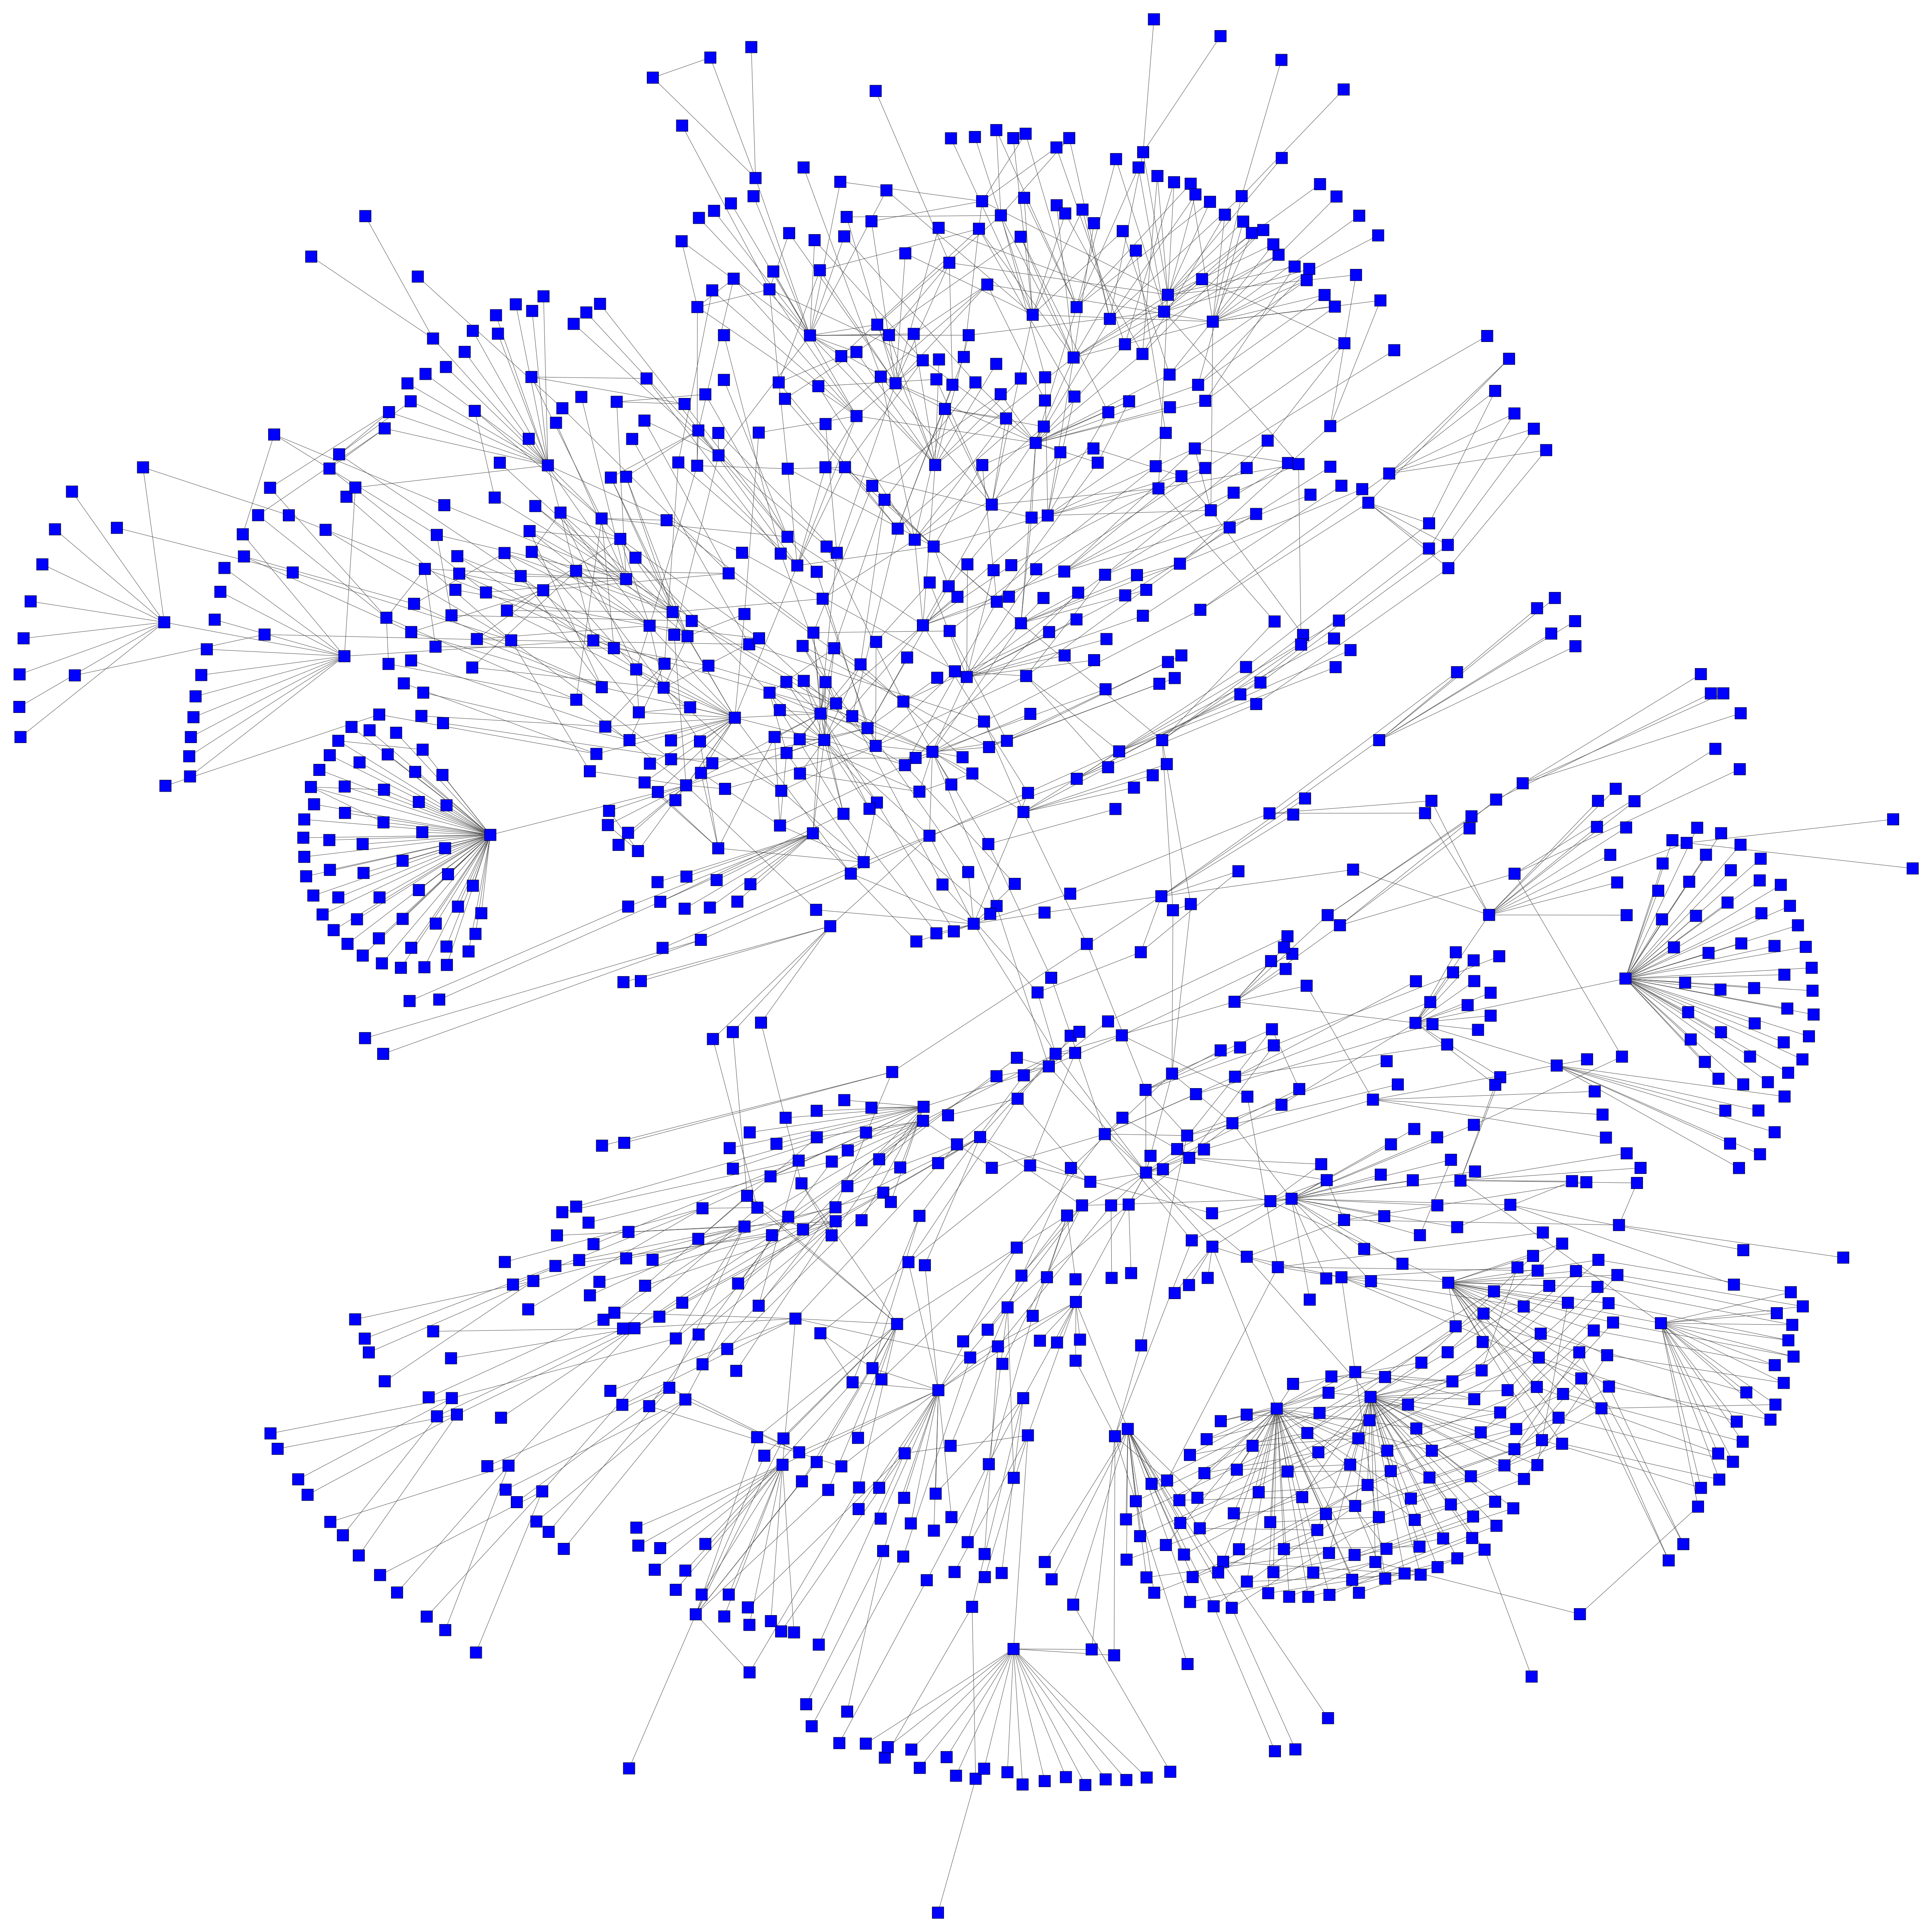
\includegraphics[width=\linewidth]{fig/graphs_category_c.png}
		\caption{Category Graph} 
		\label{fig:section2-pic2}
	\end{subfigure}
	\hspace*{\fill} % separation between the subfigures
	\begin{subfigure}{0.31\textwidth}
		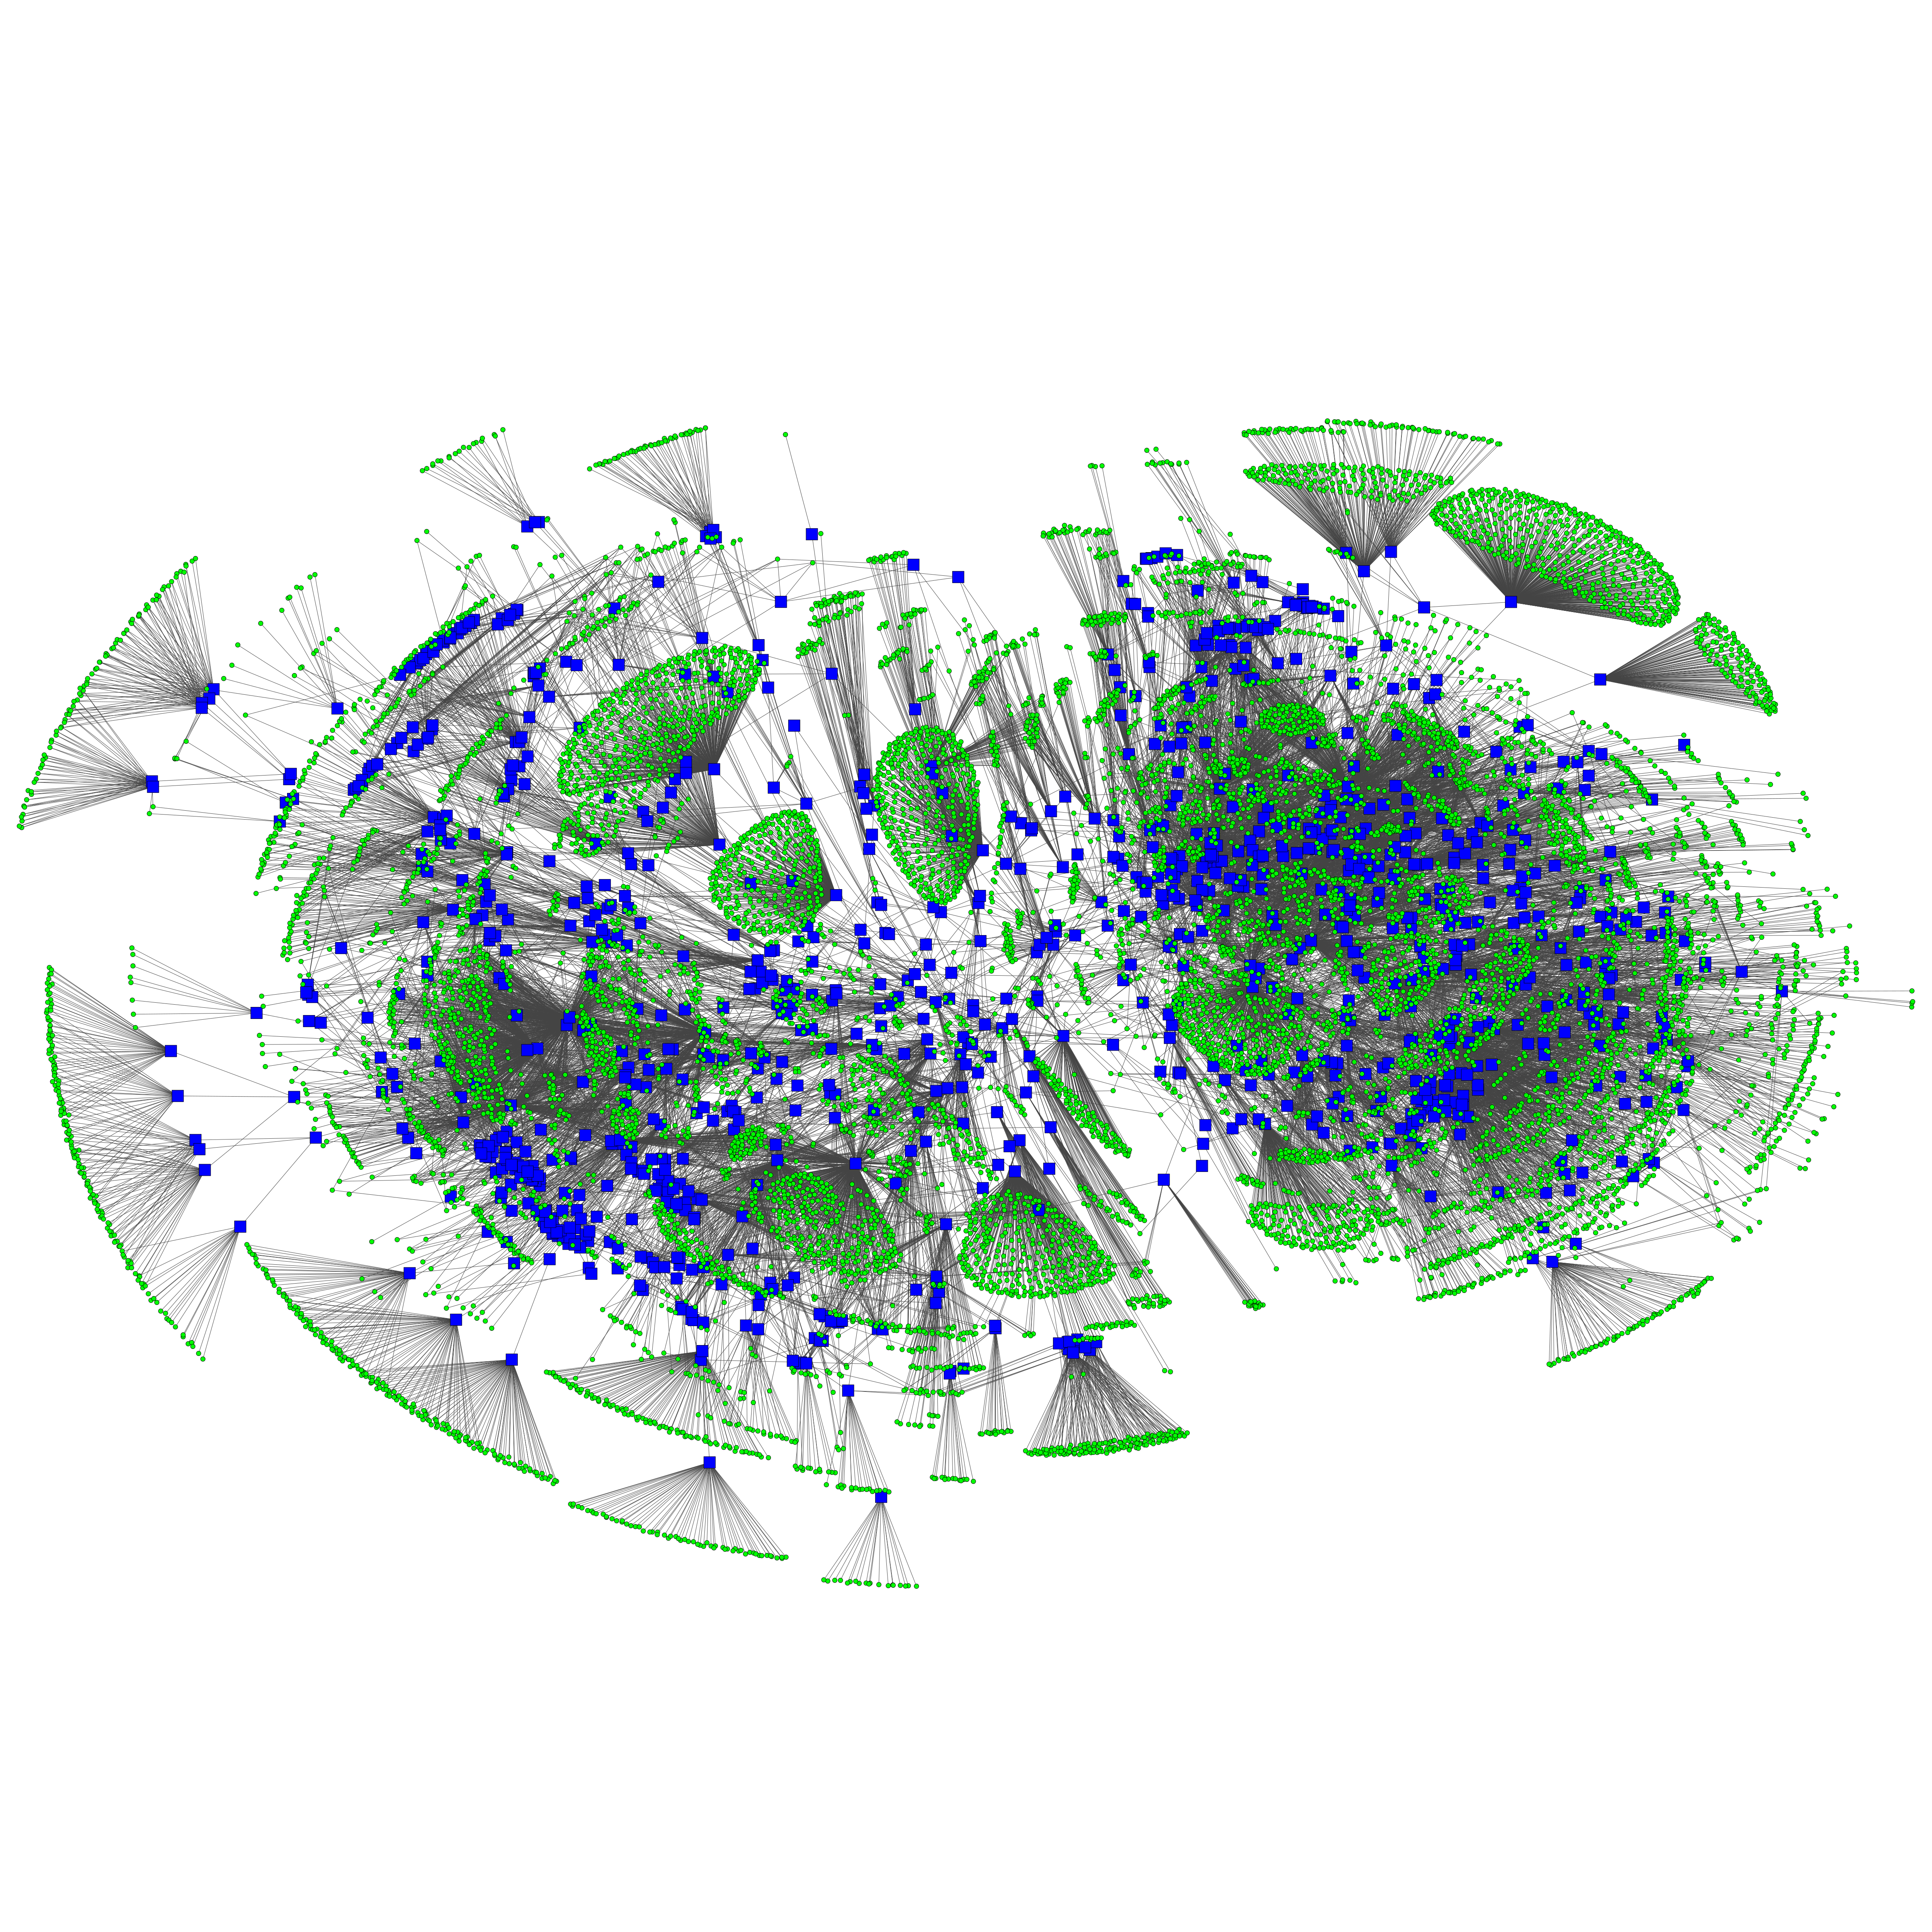
\includegraphics[width=\linewidth]{fig/graphs_category_ca.png}
		\caption{Article with Category Graph} \label{fig:section2-pic3}
	\end{subfigure}
	\hspace*{\fill} % separation between the subfigures
	\begin{subfigure}{0.31\textwidth}
		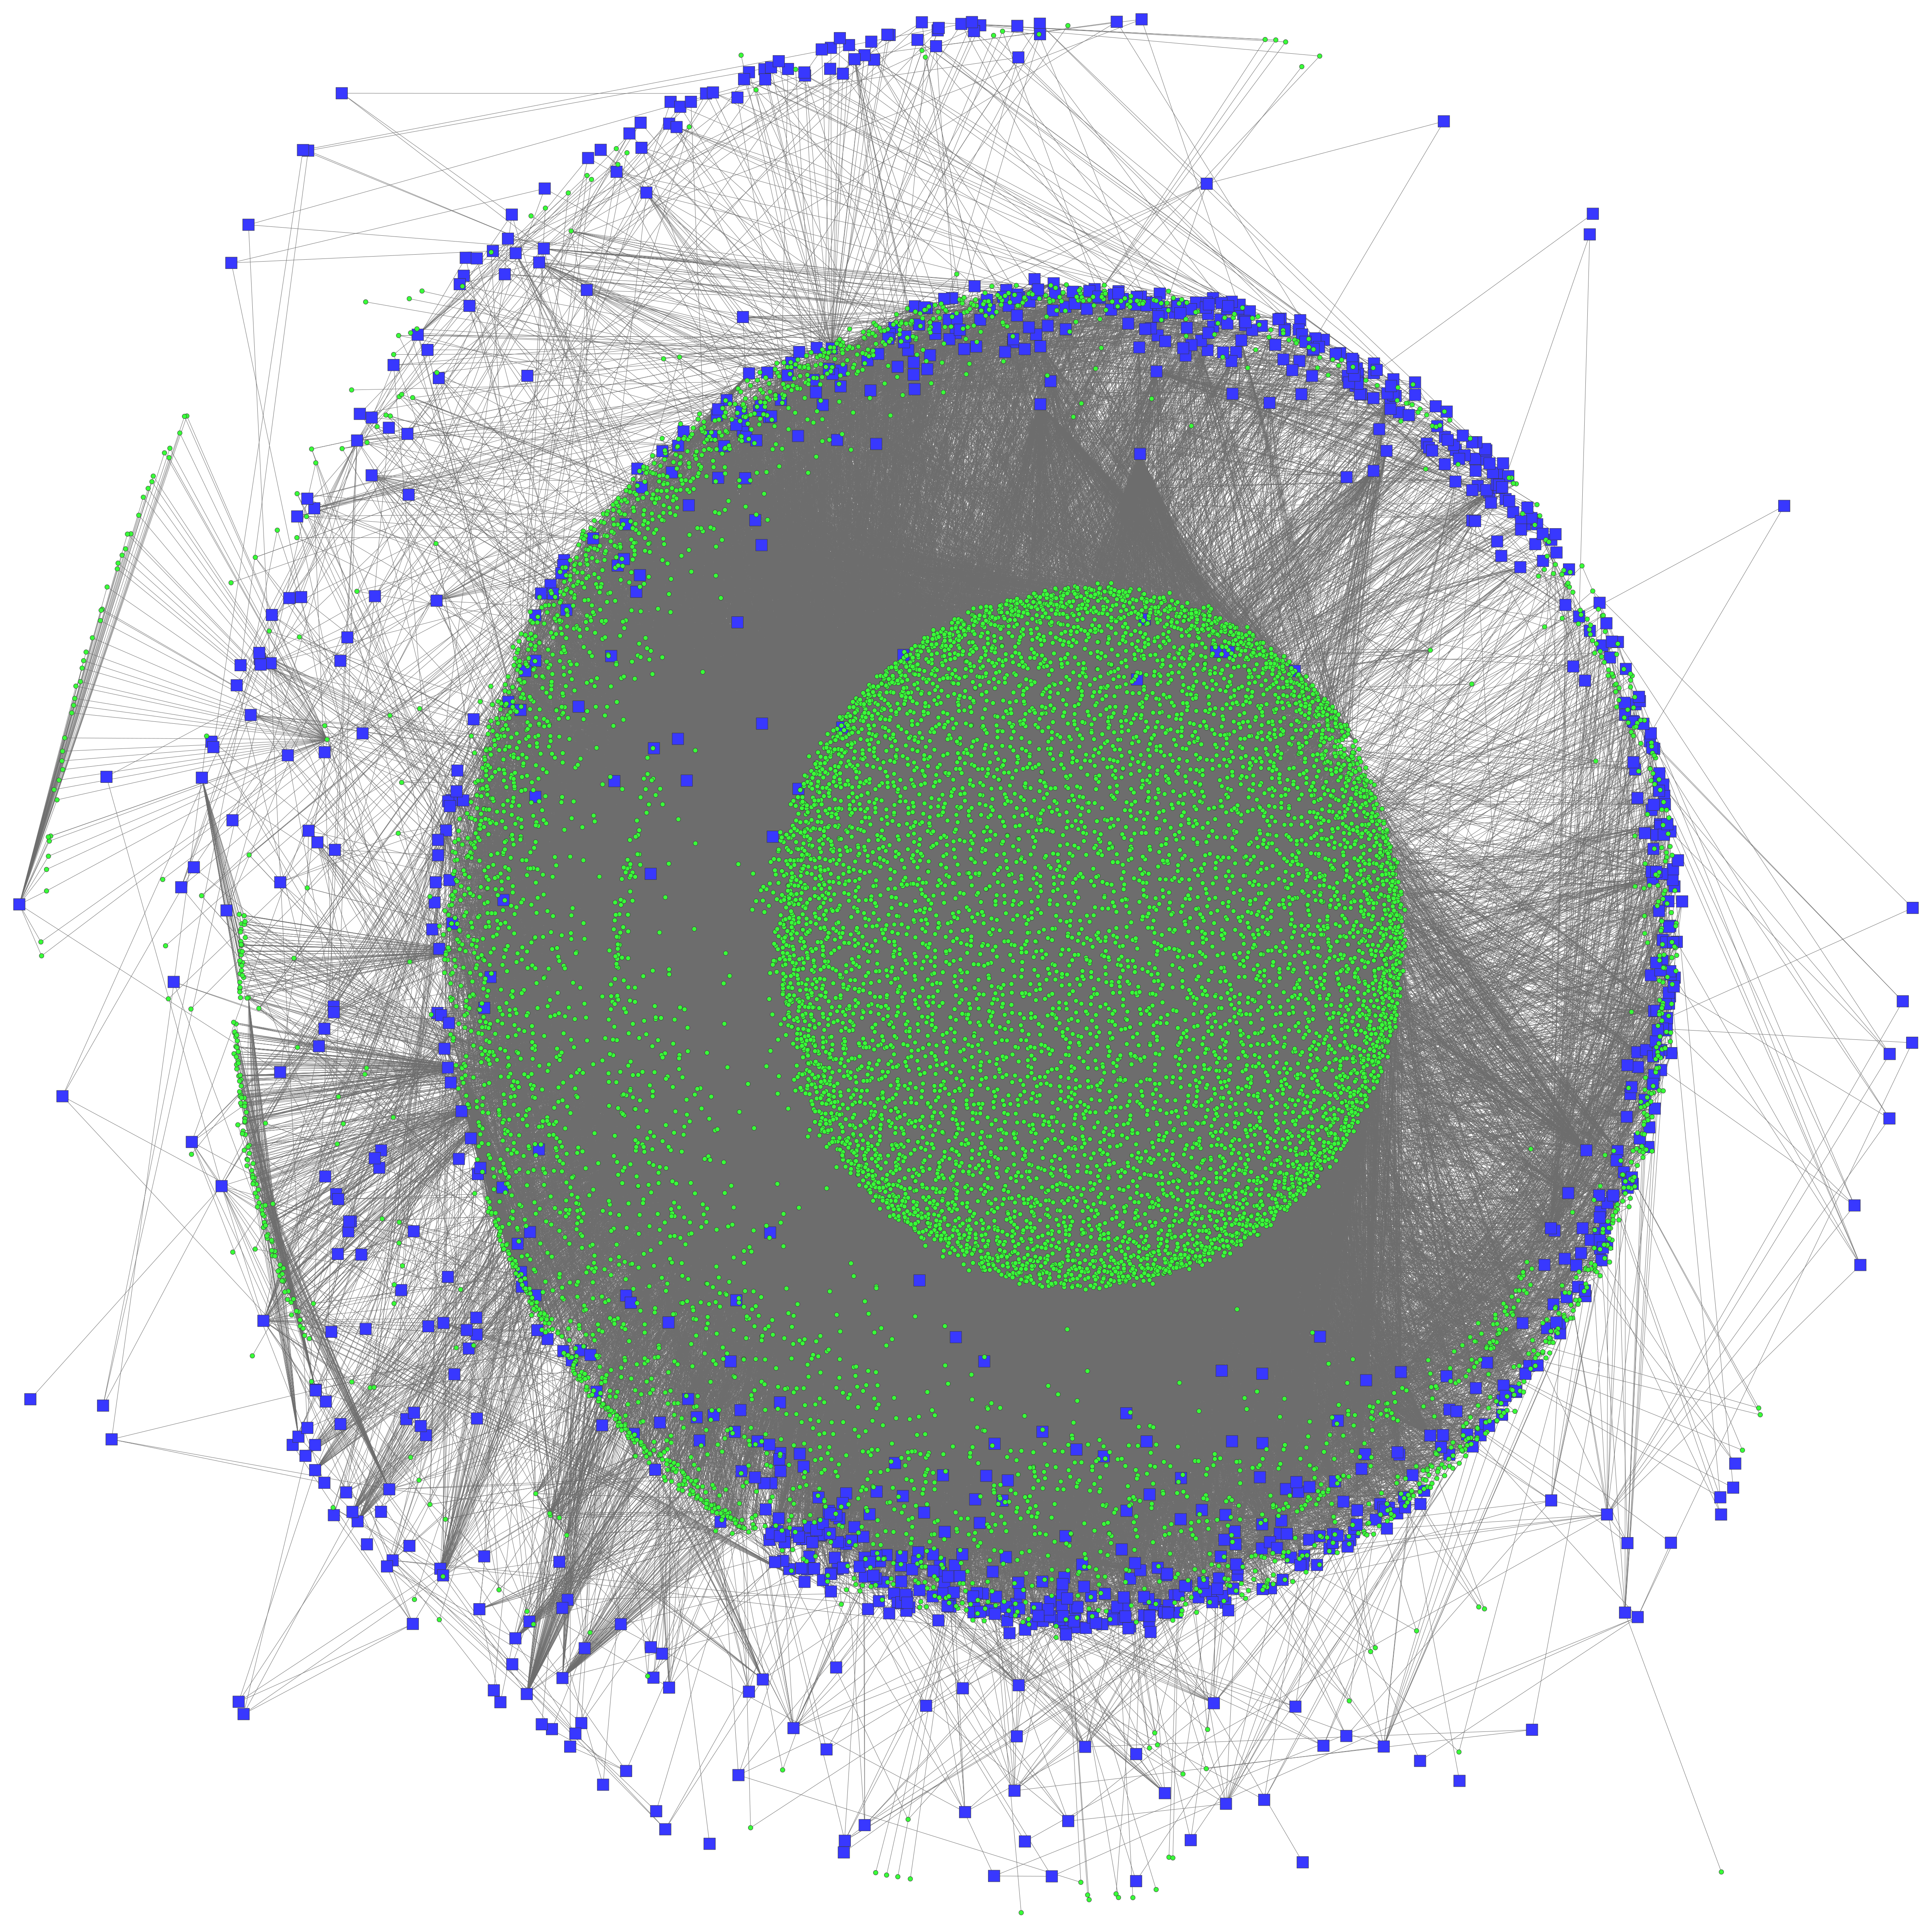
\includegraphics[width=\linewidth]{fig/graphs_category_a.png}
		\caption{Category-article Graph} \label{fig:section2-pic4}
	\end{subfigure}
	\caption{Process of Standardizing a Graph from Raw Data} \label{fig:section2-pic234}
	\vspace{-20pt}
\end{figure}

\section{Summary of Technique}
\vspace{-5pt}
\label{Ch-2:Sec:Summary of Technique}
For the original raw data, we choose the semi-structure data from \href{http://www.tolkiengateway.net}{Tolkien Gateway Website}\footnote{http://www.tolkiengateway.net} also known as TG. This is a not-for-profit collaborative wiki which aims to collect and organize the works of J.R.R. Tolkien for fans and researchers, like a Tolkien encyclopedia, while Tolkien Estate holds the copyright over the literary texts\footnote{https://en.wikipedia.org/wiki/Tolkien\_Estate}. What's more, Tolkien Gateway has become the largest and most well-built Tolkien-related encyclopedia on the World Wide Web since 2010 based on \href{http://tolkiengateway.net/wiki/List\_of\_Tolkien\_Encyclopedias}{research} by Mith\footnote{Noticing that \href{https://lotro-wiki.com/}{LOTRO-Wiki} on the top of the list with \href{https://lotro-wiki.com/index.php/Special:Statistics}{86,649 articles} is a game wiki exclusively ``\href{https://lotro-wiki.com/index.php/Lord_of_the_Rings_Online}{Lord of the Rings Online}''-related. Thus, it isn't a good choice to do the research work based on a Massively Multiplayer Online Role-Playing Game set in Tolkien's Middle-Earth.}, which gives \footnote{\href{https://lotro-wiki.com/index.php/Lord\_of\_the\_Rings\_Online}{LOTRO-Wiki}, ``\href{https://lotro-wiki.com/index.php/Special:Statistics}{Statistics}'' (retrieved 15 March 2019)}. It offers \href{http://tolkiengateway.net/w/api.php}{APIs}\footnote{Tolkien Gateway, ``\href{http://tolkiengateway.net/w/api.php}{API}'' (retrieved 15 March 2019)} with documents in detail for users to craw data from its website. The APIs are a little different from the ones of Wikipedia, so we will discuss them in the following subsections.\\
To get the raw data from a wiki farm, clean the data and change the semi-structure files into a graph, we use these techniques listed below.\\
\indent\href{https://scrapy.org/}{Scrapy}\footnote{https://en.wikipedia.org/wiki/Scrapy} is an open-source web-crawling framework which works with Python program using \href{http://www.linfo.org/bsdlicense.html}{BSD License}\footnote{https://en.wikipedia.org/wiki/BSD\_licenses}. It can be used as a data extraction with APIs or as a general-purpose web crawler\footnote{\href{https://scrapy.org/}{https://scrapy.org/}}. This framework can help us to get raw data from a wiki farm. The raw data can be set in many structures. Considering the convenience for next steps, the data is organized in Extensible Markup Language (XML). Scrapy also offers a demo frame which can help users build their own crawler.
\noindent Next, we need to extract data from the XML sources. \href{https://www.crummy.com/software/BeautifulSoup/}{BeautifulSoup} is a popular web scraping python library though a bit slow\footnote{\href{https://www.crummy.com/software/BeautifulSoup/}{https://www.crummy.com/software/BeautifulSoup/}} and \href{http://lxml.de/}{lxml} is an XML parsing library with ElementTree API\footnote{\href{http://lxml.de/}{http://lxml.de/}} though not in Python standard library. Thus, we choose to use Scrapy Selectors for data extraction. Categories (id, name), category tree and articles (id, name, detail, inner link) can be stored after this step.\\
\begin{figure*}[!tbp]
	\centering
	\def\svgwidth{0.95\columnwidth}
	\input{fig/Section2.pdf_tex}
	\caption{Process of Standardizing Graph Data}
	\label{fig:section2-pic1}
	\vspace{-25pt}
\end{figure*}
\vspace{-45pt}
Finally, we need a library to build an undirected graph with labels and attributes. igraph is an open source package with network analysis tools, well-known for its high efficiency and portability, supporting R, Python, Mathematica and C/C++.

\section{Implementation}
\vspace{-5pt}
We use demo frame of Scrapy to build three major crawlers, and get the categories, articles and the inner links between categories and articles. The process illustrated in Figure~\ref{fig:section2-pic1} will be discussed in the following sections.\\
\noindent URL crawler is labeled as jrrtgateway\_url\_scrapy in  Figure~ \ref{fig:section2-pic1}.
\vspace{-5pt}
\begin{enumerate}
	\item Focus three category roots (``Eä'', ``Real-world'' and ``Other fictional worlds'') in this wiki. Take ``Eä'' as example. Set API parameters as {action: ``query'', list: ``categorymembers'', cmlimit: 1000, format: ``xml'', cmtitle: ``Category:Eä''}. Put ``Eä'', ``Real-world'' and ``Other fictional worlds'' in stack $S$ and dictionary $L$.
	\item Pop the last item $i$ in the stack, change ``cmtitle'' to ``Category:$i$'' and run the crawler. 
	\item Extract data from XML files returned by API request and get children's ids and names (including categories, articles, files and other special pages). If a child is still a category, push the category name into the stack $S$, add category id to the key of $L$ and set category name as value. If a child is an article, article id will be added to the key of $V$ and set article name as value. Then, relationships are appended between $l$ and $l$ or $l$ and $v$ to list $E$.
	\item Repeat step 2 and 3, until stack $S$ is empty.
\end{enumerate}
\begin{table*}[!tbp]
	\label{table:parametervalues}	
	\begin{tabularx}{1.03\textwidth}{@{}cccccc@{}}
		\toprule
		Parameter & \begin{tabular}[c]{@{}c@{}}TG graph $G_L$\\ (our work)\end{tabular} & \begin{tabular}[c]{@{}c@{}}TG graph $G$\\ (our work)\end{tabular} & WCG \cite{zesch2007analysis} & WordNet \cite{miller1998wordnet} & Explanation \\ \midrule\hline
		$|V|$ & 1120 & 13332 & 27,865 & 122,005 & number of vertices \\ \hline
		$D$ & 13 & 8 & 17 & 27 & \begin{tabular}[c]{@{}c@{}}maximum eccentricity\\ of any vertex\end{tabular} \\ \hline
		$\bar{k}$ & 2.85 & 62.53 & 3.54 & 4.0 & \begin{tabular}[c]{@{}c@{}}avg number of edges\\ connected with a vertex\end{tabular} \\ \hline
		$\gamma$ & 2.66 & 1.91 & 2.12 & 3.11 & \begin{tabular}[c]{@{}c@{}}a particularity of \\scale-free network\end{tabular} \\ \hline
		$\bar{L}$ & 7.05 & 2.70 & 7.18 & 10.56 & \begin{tabular}[c]{@{}c@{}}average shortest \\path lengths\end{tabular} \\ \hline
		$\bar{L}_{random}$ & $\sim$6.70 & $\sim$2.30 & $\sim$8.10 & 10.61 & \begin{tabular}[c]{@{}c@{}}average shortest path\\ length for a random graph\end{tabular} \\ \hline
		$C$ & 0.021 & 0.25 & 0.012 & 0.027 & clustering coefficient \\ \hline
		$\bar{C}_{random}$ & 0.0087 & 17.75 & 0.0008 & 0.0001 & \begin{tabular}[c]{@{}c@{}}clustering coefficient\\ for a random graph\end{tabular} \\ \bottomrule
	\end{tabularx}
	\caption{Parameter Values of $G_L$, $G$, WCG \cite{zesch2007analysis} and WordNet \cite{miller1998wordnet}} 
	\vspace{-20pt}
\end{table*}
\vspace{-10pt}
\noindent Inner Links Crawler is labeled as jrrtgateway\_inner\_scrapy in Figure~\ref{fig:section2-pic1}.
\vspace{-5pt}
\begin{enumerate}
	\item Get article Ids $K$ from $V$ keys.
	\item Set API parameters as {action: ``query'', generator: ``links'', gpllimit: ``max'', format: ``xml'', pageids: ``$k$''} and run the crawler. 
	\item Extract inner link nodes and add the relationships between vertices to edges $E$.
	\item Repeat Step 2 and 3, until get all article inner links.
\end{enumerate}
%\vspace{10pt}

\noindent Article Crawler is labeled as jrrtgateway\_article\_scrapy in Figure~\ref{fig:section2-pic1}.
\vspace{-5pt}
\begin{enumerate}
	\item Get article Ids $K$ from $V$ keys.
	\item Set API parameters as {action: ``query'', generator: ``links'', gpllimit: ``max'', format: ``xml'', pageids: ``$k$''} and run the crawler. 
	\item Extract inner link nodes and add the relationships between vertices to edges $E$.
	\item Repeat Step 2 and 3, until get all article inner links.
\end{enumerate}

\indent Finally, we merge the clean data extracted from the results of three crawlers shown in Figure~\ref{fig:section2-pic234}. We also calculate the graph parameters of $G_L$ and $G$ listed in Table 2.1. The parameters from the paper of WCG \cite{zesch2007analysis} are number of vertices $|V|$, diameter $D$, average degree $\bar{k}$, power law exponent $\gamma$ \cite{doi:10.1080/00107510500052444} \cite{clauset2009power}, average shortest path length $\bar{L}$, average shortest path length for a random graph $\bar{L}_{random}$ \cite{watts1998collective}, clustering coefficient $C$ \cite{wasserman1994social} and clustering coefficient for a random graph $\bar{C}_{random}$ \cite{zlatic2006wikipedias}.

%\section{Graph-theoretic Analysis}
%\label{Ch-2:Sec:Analysis of Graph}

%After the graph standardization, we need to analyze whether $G_L$ meets the particularities of scale-free, small world graphs. If the answer is ``yes'', the algorithms which works for WCG can be transferred to $G_L$. The parameters (listed in \cite{zesch2007analysis}) are number of vertices $|V|$, diameter $D$, average degree $\bar{k}$, power law exponent $\gamma$ (\cite{newman2005power}, \cite{clauset2009power}), average shortest path length $\bar{L}$, average shortest path length for a random graph $\bar{L}_{random}$ (\cite{watts1998collective}), clustering coefficient $C$ (\cite{wasserman1994social}) and clustering coefficient for a random graph $\bar{C}_{random}$ (\cite{zlatic2006wikipedias}). The parameter values for WCG are quoted from \cite{zesch2007analysis}, while values for WordNet are from according to \cite{steyvers2005large}.



%\section{Conclusion}
%As $G_L$ is a semantic network and follows a power law, $G_L$ is a scale-free graph. From the results of $G_L$ in \nameref{table:parameter values}, we can see that small values of $\bar{L} \gtrsim \bar{L}_{random}$ with large values of $C \gg C_{random}$ (\cite{zesch2007analysis}). $G_L$ meets the characteristics of small-world graphs which can be used for natural language processing tasks. \\
%What's more, article graph $G_V$ is a heavily linked semantic networks. After adding $G_V$ to $G_L$, its degree distribution still follows a power law, with $\gamma = 2.01$. Thus, $G$ is a scale-free graph, with a small-word label graph and a heavily linked article graph.
